\documentclass{article}
\usepackage{amsmath}
\usepackage{amssymb}
\usepackage{algorithm}
\usepackage{float}
\usepackage{color}
\usepackage{multicol}
\usepackage{forloop}
\usepackage{graphicx}
\usepackage[margin=0.8in]{geometry}
\usepackage{caption}
\usepackage{enumerate}

\graphicspath{ {.} }
\title{MATH 3800 F\\
	\large{Assignment 1}}
\author{Krystian Wojcicki, 101001444}
\date{Winter 2020}

\begin{document}
\maketitle

\begin{enumerate}[1.]
\item

\textbf{Verify that $f(x) = x^3 +8x - 7$ has a root in $[0,1]$.  Use fixed-point iteration to find this
root to 5 decimal places. Start with $x_0 = 0.75$, but verify that your chosen $g(x)$ will work
before you begin.:}

First verify that $f(a) * f(b) < 0$. \\
$f(0) = 0^3 + 8 * 0 - 7 = -7, f(1) = 1^3 + 8 * 1- 7 = 2 \to f(a) * f(b) \to -7 * 2 < 0$. \\
Therefore since there is a sign change there must also be a root in the interval $[0,1]$.

$f(x) = x^3 + 8x - 7 \to \frac{7 - x^3}{8}$. Take $g(x) = \frac{7 - x^3}{8}$

Since $|g\prime(x)| = |\frac{-3x^2}{8}| = |-\frac{3}{8}x^2|  \leq \frac{3}{8} < 1$ on $[0,1]$ then $x_{n+1} = g(x_n)$ will generate a convergent sequence.

\begin{gather*}
x_0 = 0.75, x_1 = g(0.75) = \frac{7 - 0.75^3}{8} = 0.82227 \\
x_2 = g(0.82227) = 0.80551 \\
x_3 = g(0.80551) = 0.80967 \\
x_4 = g(0.80967) = 0.80865 \\ 
x_5 = g(0.80865) = 0.80890 \\
x_6 = g(0.80890) = 0.80884 \\
x_7 = g(0.80884) = 0.80885 \\
x_8 = g(0.80885) = 0.80885
\end{gather*}

Check $f(0.80885) \simeq -0.00002$ therefore very close to 0 and the root is 0.80885.

\item
\textbf{Use Newton’s Method to find the point of intersection of the curves $y = x^3$ and $y = cos(x)$ to 6 decimal places. Start with $x_0 = 1$:}

If $x^3 = cos(x)$ then $f(x) = x^3 - cos(x) = 0$. So $f\prime(x) = 3x^2 + sin(x)$.

So $x_{n+1} = x_n - \frac{f(x_n)}{f\prime(x_n)} = x_n - \frac{x^3 - cos(x)}{3x^2 + sin(x)} = \frac{2x^3 + x * sin(x) + cos(x)}{3x^2 + sin(x)}$

\begin{gather*}
x_0 = 1, x_1 = \frac{2* 1^3 + 1 * sin(1) + cos(1)}{3 * 1^2 + sin(1)} = 0.880333 \\
x_2 = g(0.880333) = 0.865684 \\
x_3 = g(0.865684) = 0.865474 \\
x_4 = g(0.865474) = 0.865474 \\
\end{gather*}

Check $f(0.865474) \simeq -9.96 * 10^{-8}$ which is very close to 0 therefore okay and the root solution to the intersection of the curves is $x = 0.865474$.

\item
\textbf{Solve the following dynamical systems. Find and classify any equilibria.:}

Firstly we know that when $a_{n+1} = r*a_n + b$ then $a_n = r^n(a_0 - a) + a, a = \frac{b}{1-r}$ if $r \neq 1$.

\begin{enumerate}[(a)]
  \item \textbf{$a_{n+1} = (2/5)a_n, a_0 = 10$:} 
$\to b = 0, r=2/5 \to a = \frac{0}{1 - r} \to a = 0$. Therefore the solution is $a_n = (2/5)^n(10)$ and the equilibrium is when $a = 0$.

  \item \textbf{$a_{n+1} = (3/5)a_n + 100, a_0 = 20$:}
$\to b = 100, r = 3/5 \to a = \frac{100}{1 - 3/5} = 250$. Therefore the solution is $a_n = (3/5)^n(20 - 250) + 250$ and the equilibrium is when $a = \frac{100}{1 - 3/5} = 250$.

  \item \textbf{$a_{n+1} = (-2/3)a_n + 500, a_0 = 25$:} 
$\to b = 500, r=-2/3 \to a = \frac{500}{1 - -2/3} \to a = 300$. 
Therefore the solution is $a_n = (-2/3)^n(25 - 300) + 300$ and the equilbirium is when $a = \frac{500}{1 - -2/3} = 300$.

  \item \textbf{$a_{n+1} = 3a_n - 30, a_0 = 0$:} 
$\to b = -30, r=3 \to a = \frac{-30}{1 - 3} \to a = 15$. Therefore the solution is $a_n = 3^n(0 - 15) + 15$ and the equilibrium is when $a = \frac{-30}{1-3} = 15$.
\end{enumerate}

\item 
\textbf{Suppose that Owls have Mice for their primary food source in a wildlife sanctuary. If $M_n$ is the Mouse population after $n$ years and $O_n$ is the Owl, the following model has been suggested:}

\begin{gather*}
M_{n+1} = 1.3M_n - 0.002O_nM_n \\
O_{n+1} = 0.6O_n + 0.0004O_nM_n
\end{gather*}

\begin{enumerate}[(a)]
\item
\textbf{What type of interaction is this ? How do the coefficients tell us ?:} \\
$M_{n+1} = \underbrace{1.3}_{\text{Mouse population grows if no owls}}M_n - \underbrace{0.002}_{\text{Mouse population decreases with presence of owls}}O_nM_n$ \\
$O_{n+1} =  \underbrace{0.6}_{\text{Owl population decreases if no mice}}O_n + \underbrace{0.0004}_{\text{Owl population increased by presence of mice}}O_nM_n$ \\

Based on the coefficients this is a predator prey interaction.
\item
\textbf{Find the equilibrium values ?}
As taught in class when we have a system of equtions as follows:
\begin{gather*}
x_{n+1} = ax_n-bx_ny_n \\
y_{n+1} = cy_n + dx_ny_n
\end{gather*}

Then the system has two fixed points (0,0) and $(\frac{1-c}{d},\frac{a-1}{b})$. 

In our case this gives equilibrium values of $(\frac{1-c}{d},\frac{a-1}{b}) \to (\frac{1 - 0.6}{0.0004}, \frac{1.3 - 1}{0.002}) \to (1000, 150)$ and the solution $(0,0)$. 
\item
\textbf{Predict the long-term outcome if $M_0 = 1200$ and $O_0 = 100$}
\\
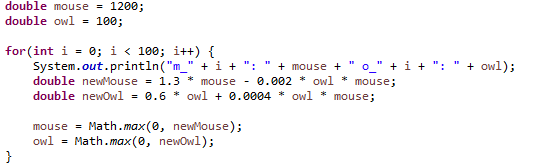
\includegraphics{mousecode} \\
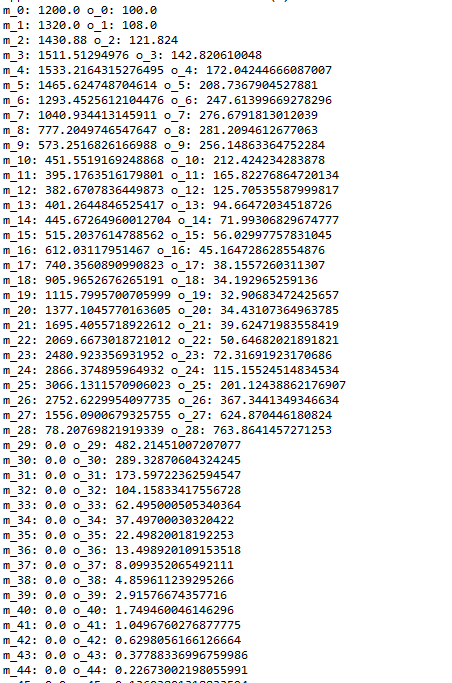
\includegraphics{mouseoutput_p1} \\ 
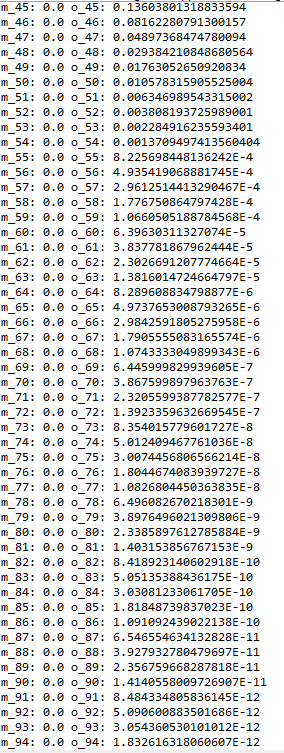
\includegraphics{mouseoutput_p2} \\
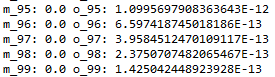
\includegraphics{mouseoutput_p3} \\

As can be seen from the above screenshots. There is first some cycling in the populations and at $n = 29$ the mice are completely wiped out, afterwards the owls die off as well due to the fact there are no mice left.

\end{enumerate}

\end{enumerate}
\end{document}